\chapter{Einleitung}

\begin{fquote}[Mark Zuckerberg][Facebook CEO][2014]
Virtual reality was once the dream of science fiction. But the internet was also once a dream, and so were computers and smartphones. The future is coming.
\end{fquote}

\begin{fquote}[Tim Cook][Apple CEO][2017]
I think AR is [...] big, it’s huge. I get excited because of the things that could be done that could improve a lot of lives.
\end{fquote}

\section{Einführung}
Viele der einflussreichsten Technologieunternehmen arbeiten an der \emph{Virtual} bzw.\ \emph{Augmented Reality (VR} bzw.\ \emph{AR)}. Tim Cook ist überzeugt davon, dass die AR die nächste \emph{``big idea''} nach dem Smartphone wird. \cite{theindependent2017apple}

Nicht nur Großkonzerne wie Apple, Facebook oder Samsung arbeiten intensiv in diesem Bereich. Ein Start-up-Unternehmen namens \emph{Magic Leap} entwickelt eine AR Brille und wird von Investoren in Billionenhöhe unterstützt. \cite{kelly2016untold} Laut einem Cover-Artikel der Zeitschrift \emph{Wire} ist die noch unter Verschluss gehaltene Technologie den Konkurrenzprodukten allen voraus. Das Release der Hardware ist Stand heute noch nicht bekannt, aber es lässt sich ein Trend erkennen, der die nächsten Jahre viele neue Möglichkeiten eröffnen wird und möglicherweise die Digitalisierung revolutionieren könnte.
Diese Arbeit wird sich mit einer Anwendung für die AR beschäftigen -- der Softwarevisualisierung. Die Spezialisierung auf AR kann nach der Abgrenzung von AR und VR besser nachvollzogen werden.

\paragraph{VR} ist eine Umgebung, in der der Betrachter vollkommen von einer computergenerierten Welt umgeben ist, die oft die reale Welt imitiert, aber auch rein fiktiv sein kann. \cite{milgram1995augmented}\\

Obwohl der Begriff AR zunehmend in der Industrie Verwendung findet, entbehrt er doch einer einheitlichen Definition. In \cite{azuma1997survey} wird AR als \emph{"`Variation"'} von VR betrachtet. Dagegen vermittelt Milgrim in \cite{milgram1995augmented} ein vollständigeres Verständnis, weshalb sich die Begrifflichkeiten in dieser Arbeit daran anlehnen sollen. Nach Milgrim existieren die beiden entgegengesetzten Extreme der Realität und der Virtualität. Alles dazwischen ist die sogenannte \emph{Mixed Reality (MR)}.

\paragraph{MR} ist eine Umgebung, in der Elemente der realen und einer virtuellen Welt zusammen dargestellt werden.\\

\begin{figure}[htb]
  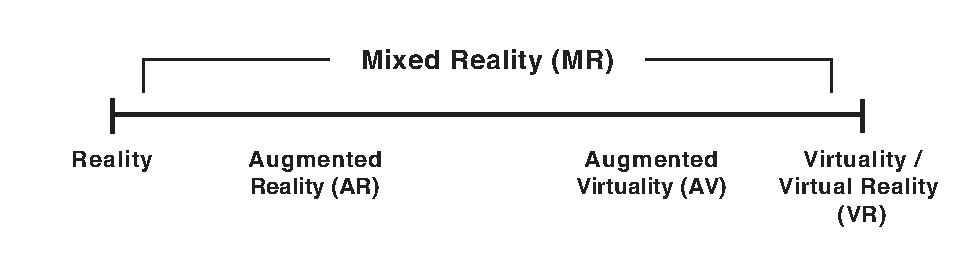
\includegraphics[width=.8\textwidth]{\figdir/rv-continuum}
  \caption{Abgewandelte Darstellung des Reality-Virtuality-Kontinuums aus \cite{milgram1995augmented}}
  \label{fig:rv-continuum}
\end{figure}

Dieses \emph{Reality-Virtuality-Kontinuum} ist in Abbildung \ref{fig:rv-continuum} dargestellt, in dem gut zu erkennen ist, dass AR zu der Mixed Reality gehört. In den meisten Quellen wie \cite{azuma1997survey}\cite{azuma2001recent}\cite{kato1999marker} wird bei der AR noch die Komponente der Interaktion aufgeführt. AR kann deshalb folgendermaßen definiert werden:

\paragraph{AR} ist die Erweiterung der realen Welt durch computergenerierte Elemente, mit denen der Betrachter in Echtzeit interagieren kann.\\

Auch die \emph{Augmented Virtuality}, also die Erweiterung der virtuellen Welt durch reale Elemente, gehört zur MR.

Wie viele der einflussreichsten Menschen der Technologie-Industrie, sieht Tim Cook  mehr Zukunft in der AR, da, wie er in einem Interview sagt, diese Technologie nicht wie die VR die wirkliche Welt ausschließt, sondern die Realität erweitert und Teil von zwischenmenschlicher Kommunikation sein kann. \cite{theindependent2017apple}

Wir stellen uns ein Hologramm vor, dass auf einem Konferenztisch Gestalt annimmt und ein Software-System repräsentiert. Entwickler, Projektleiter oder auch Kunden versammeln sich um den Tisch und können miteinander interaktiv die Software betrachten, evaluieren und wichtige Informationen daraus ziehen.

Dies wäre mit VR nicht möglich, da der Betrachter von der Außenwelt abgeschottet ist. Deshalb wird im Zuge dieser Arbeit mit der Stand heut am weitesten ausgereiften Technologie der AR gearbeitet -- der \emph{HoloLens} von Microsoft.

\section{Motivation dieser Arbeit}
Die Technologie der AR bietet uns viele neue Möglichkeiten. Eine Motivation dieser Arbeit ist es sich produktiv mit einer neuen, zukunftsträchtigen Technologie zu beschäftigen. Das ist jedoch nur die eine Seite. Die weitaus größere Motivation ist, die zuvor noch nicht dagewesene Zugänglichkeit und Interaktion mit dreidimensionaler \emph{Visualisierung} auszunutzen. Visualisierung im Allgemeinen begegnet uns in vielen Bereichen unseres Lebens und nimmt eine wichtige Rolle ein.

Niemand konnte bislang unser Sonnensystem von außen betrachten. Dennoch haben wir alle eine ziemlich gute Vorstellung wie dieses aufgebaut ist. Durch die Visualisierung der Planeten und der Sonne entsteht in uns ein geistiges Abbild der Realität. Das Konzept komplexe Realitäten zu abstrahieren und zu visualisieren, um dadurch die Realität besser verstehen zu können, ist in vielen Disziplinen der Wissenschaft vertreten.

Neben Wissenschaften wie Physik, Chemie oder Biologie, nimmt Visualisierung
auch besonders in der Informatik eine wichtige Rolle ein. In vielen Bereichen müssen Informationen in eine visuelle Form gebracht werden, die für das menschliche Auge besser zu lesen sind.

Gerade bei komplexen Software-Systemen ist das der Fall. Soll zum Beispiel die zu Grunde liegende Struktur einer Software Außenstehenden erklärt werden, gelingt das mit einem visuellen Modell wie einem UML-Diagramm sicherlich besser, als nur in den Source-Code zu schauen.

So wie UML-Diagramme, war die Darstellungsform der Softwarevisualisierung bislang meist zweidimensional. Mit AR wird dieser Disziplin der Visualisierung jedoch wortwörtlich ein neuer Raum an Möglichkeiten eröffnet und in diese Arbeit soll diesen Raum ausfüllen.

\section{Zielsetzung}
Für die Zielsetzung einer 3D Softwarevisualisierung in der AR sollten zunächst die allgemeinen Ziele einer Softwarevisualisierung betrachtet werden. Softwarevisualisierung ist für Diehl die "`visualization of artifacts related to software and its development process"' \cite{diehl2007software}. Wird aber der Fokus mehr auf die Ziele, d.h. den Nutzen für den Betrachter gelegt, lässt sich Softwarevisualisierung wie folgt definieren:

\begin{quotation}
Softwarevisualisierung ist die bildliche oder auch metaphorische Darstellung einer Software, um dem Betrachter durch Vereinfachung und Abstraktion das bessere Verständnis oder die einfachere Analyse von Software zu ermöglichen.
\end{quotation}

In dieser Arbeit soll das neue Konzept \emph{CodeLeaves} für eine solche Softwarevisualisierung in der AR vorgestellt und im Detail ausgearbeitet werden.

Dabei soll CodeLeaves, im Vergleich zu andern 3D Softwarevisualisierungen, die Vorteile der Dreidimensionalität optimal ausnutzen.

Im Vorfeld dieser Arbeit wurden in einer Studie Metriken gesammelt, die eine gute Softwarevisualisierung bzw. CodeLeaves unterstützen sollte.

Es sollen dynamische und statische Metriken zur Erkennung von Anomalien in einer Software unterstützt werden. Ebenfalls soll die Darstellung der Struktur und der darauf abgebildeten Abhängigkeiten innerhalb einer Software möglich sein.

Durch weitere Expertengespräche sollen Userstories erstellt werden um zu den Mehrwert des neuen Konzepts validieren zu können.

Um diesen Anforderungen gerecht zu werden, soll für CodeLeaves ein sprachunabhängiges Datenmodell entworfen werden, dass alle geforderten Metriken unterstützt.

Der Praktische Teil dieser Arbeit soll die prototypische Entwicklung von CodeLeaves für die HoloLens sein.

\section{Aufbau der Arbeit}
Im Kapitel \ref{ch:concept} wird das Konzept von CodeLeaves vorgestellt. Dabei wird zunächst unter Betrachtung alternativer Ansätzen begründet, wieso ein neues Konzept sinnvoll ist, um dann in Abschnitt \ref{sec:idea} genauer auf das Konzept einzugehen. Die Befragung von Experten der Softwareanalyse und die daraus abgeleiteten Anforderungen an CodeLeaves in Abschnitt \ref{sec:requirements} schließen das erste Kapitel ab.

Das Kapitel \ref{ch:data-model} beschäftigt sich mit der Entwicklung eines geeigneten Datenmodells für CodeLeaves. Es werden vorhandene Datenmodelle auf Tauglichkeit für CodeLeaves überprüft und Rücksprache mit erfahrenen Software-Ingenieuren gehalten.

Aufbauend auf das entwickelte Datenmodell, wird das Konzept von CodeLeaves in Kapitel \ref{ch:modelling} theoretisch weiter ausgearbeitet. Darunter fällt die Positionierung der Bäume auf einer Grundfläche und die Länge, Dicke und der Winkel der einzelnen Äste. Parallel zur Theorie wird aufgezeigt, wie sich CodeLeaves in Unity für die HoloLens modellieren lässt.

Die Interaktion mit CodeLeaves soll Thema des Kapitel \ref{ch:interaction} sein. Besonders die Abhängigkeiten von Artefakten einer Software sollen mithilfe von CodeLeaves interaktiv exploriert werden können.

Das Kapitel \ref{ch:conclusion} fasst die Ergebnisse der Arbeit zusammen und ein Ausblick auf zukünftige Verwendung und weiterführende Arbeiten runden die Arbeit ab.

\chapter{Das Konzept CodeLeaves}
\label{ch:concept}

``Hierarchies are almost ubiquitous [...]'' \cite{robertson1991cone} haben Robertson et. al schon 1991 bei der Visualisierung von hierarchischen Informationen festgehalten. So auch bei der Struktur einer Software. Jede Software mit einer geschachtelten Paketstruktur ist hierarchisch und ist in einer Baumstruktur angeordnet. Die Dateien der Software bilden die Blätter.

Der in der Informatik selbstverständlich verwendete Begriff "`Blätter"' zeugt von der ursprünglichen Metapher der Baumstruktur -- ein dreidimensionaler Baum wie er in der Natur wächst. Für eine 3D Softwarevisualisierung legt das eine wortwörtliche Interpretation der Baum-Metapher nahe.

\section{Vergleich mit anderen Konzepten}
\label{sec:comparison}
\section{Grundliegende Idee der Metapher Software-Wald}
\label{sec:idea}
\section{Anforderungen an CodeLeaves}
\label{sec:requirements}

\chapter{Datenmodell}
\label{ch:data-model}
\section{FAMIX-Familie}

\chapter{Modellierung}
\label{ch:modelling}

\chapter{Interaktionskonzept}
\label{ch:interaction}
\chapter{Zusammenfassung und Ausblick}
\label{ch:conclusion}
